\chapter{Zadatak F} \label{ch:f}

U ovom poglavlju je opisan i odrađen zadatak F.

\section{Opis zadatka} \label{sec:f:opis}

na temelju podataka iz d) dijela zadatka, potrebno je odrediti svaku komponentu mehaničke energije
potrebne za savladavanje otpora na temelju fizikalne slike vozila. Potrebno je prikazati krivulje svake
komponente mehaničke energije zasebno i sve na jednom grafu s točno naznačenim oznakama.
Dodatno, za svaku komponentu energije je potrebno odrediti minimalnu, maksimalnu i srednju
vrijednost krivulje, te prikazati je u tabličnom obliku

\section{Rješenje} \label{sec:f:rjesenje}

Za riješavanje ovog zadatka potrebno je izračunati pomnožiti sve snage iz zadatka d sa vremenom.
Nakon toga potrebno je obaviti \textit{scan\_sum} operaciju nad svim energijama kako bi se dobila
ukupna energija.

\begin{figure}
    \centering
    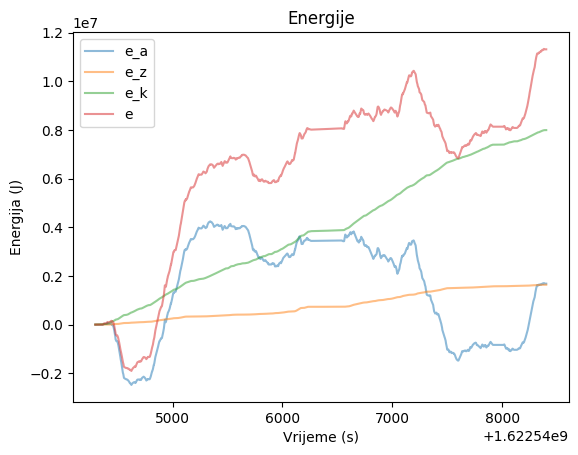
\includegraphics[width=0.8\textwidth]{images/energies.png}
    \caption{Prikaz izračunate energije kroz vrijeme.}
    \label{fig:f:energy_graph}
\end{figure}


\begin{table}[!ht]
    \centering
    \caption{Analiza energija na vozilu}
    \begin{tabular}{lllll}
    \hline
        \textbf{describe} & \textbf{e\_a} & \textbf{e\_z} & \textbf{e\_k} & \textbf{e} \\ \hline
        """count""" & 9776.0 & 9776.0 & 9776.0 & 9776.0 \\ 
        """null\_count""" & 0.0 & 0.0 & 0.0 & 0.0 \\ 
        """mean""" & 1.5759e6 & 789315.717893 & 3.9534e6 & 6.3186e6 \\ 
        """std""" & 2.0992e6 & 528533.332128 & 2.3441e6 & 3.3057e6 \\ 
        """min""" & -2.4799e6 & 0.0 & 0.0 & -1.9022e6 \\ 
        """25\%""" & -795646.262964 & 380748.85302 & 2.2792e6 & 5.9182e6 \\ 
        """50\%""" & 2.5803e6 & 732464.143333 & 3.8511e6 & 7.5995e6 \\ 
        """75\%""" & 3.4450e6 & 1.3209e6 & 6.0400e6 & 8.1365e6 \\ 
        """max""" & 4.2387e6 & 1.6376e6 & 7.9961e6 & 1.1334e7 \\ \hline
    \end{tabular}
    \label{table:c:energies}
\end{table}